% Created 2016-12-02 Fri 17:30
% Intended LaTeX compiler: pdflatex
\documentclass[11pt]{article}
\usepackage[utf8]{inputenc}
\usepackage[T1]{fontenc}
\usepackage{graphicx}
\usepackage{grffile}
\usepackage{longtable}
\usepackage{wrapfig}
\usepackage{rotating}
\usepackage[normalem]{ulem}
\usepackage{amsmath}
\usepackage{textcomp}
\usepackage{amssymb}
\usepackage{capt-of}
\usepackage{hyperref}
\author{Max T. Curran and Nick Merrill}
\date{\today}
\title{One-step, three-factor authentication with in-ear EEG}
\hypersetup{
 pdfauthor={Max Curran and Nick Merrill},
 pdftitle={One-step, three-factor authentication with in-ear EEG},
 pdfkeywords={},
 pdfsubject={},
 pdfcreator={Emacs 26.0.50.2 (Org mode 9.0.1)}, 
 pdflang={English}}
\begin{document}

\maketitle
\begin{abstract}
We propose the first research study of one-step three-factor authentication.
Specifically we seek to demonstrate its feasibility and quantify its performance
using Ear EEG (electroencephalogram). By performing a single mental task, our
user will be able to present three authenticators at once – a knowledge factor
(their chosen secret thought and/or mental task), an inherence factor (their
brainwave signals), and a possession factor (the EEG sensing earpiece that is
custom-fitted to their ear). We will build the custom-fit Ear EEG earpieces and
conduct an experimental study to evaluate the accuracy and usability of this
authentication method.
\end{abstract}
\section{Introduction and Motivation}
\label{sec:org5c92f27}

It is well appreciated by experts and end-users alike that strong authentication is
critical to cybersecurity and privacy, now and into the future. Unfortunately,
news reports of celebrity account hackings serve as regular reminders that
the currently dominant method of authentication in consumer applications, 
single-factor authentication using passwords or other user-chosen secrets, 
is faced by many challenges. Major industry players such as Google and
Facebook have been strongly encouraging their users to adopt two-factor
authentication (2FA). However, the need for users to submit two different 
authenticators in two separate steps has frustrated wide adoption, 
due its additional hassle cost to the users. For instance, the popular Apple
iPhone has already implemented the necessary technologies to support device
unlock using either a user-selected passcode or a fingerprint. Therefore the
device could easily support a two-step two-factor authentication scheme if
desired. However, it is easy to understand why users would balk at having to
enter a passcode \emph{and} provide a fingerprint each time they want to unlock their phone.

In previous work, “one-step two-factor authentication” has been proposed as a
new approach to authentication that can provide the security benefits of two-
factor authentication without incurring the hassle costs of two-step verification [1].
By employing consumer-grade EEG (electroencephalogram) sensing
technologies, it was demonstrated in a 2013 passthoughts study that a user can
submit both a knowledge factor (i.e., secret thought) and an inherence factor
(i.e., brainwave signal unique to the individual) in a single step by performing a
single mental task [2]. Additionally, the robustness of this method against
impersonation attacks was demonstrated, including conditions where the attacker
may have learned the target’s secret thought and/or secret task [3].

In the present proposal, we will undertake, to the best of our knowledge, the first
ever study of one-step three-factor authentication. In computer security,
authenticators are classified into three types: knowledge factors (e.g., passwords
and PINs), possession factors (e.g., physical tokens, ATM cards), and inherence
factors (e.g., fingerprints and other biometrics). Because three-factor
authentication (3FA) requires the user to submit one distinct instance of each
type of authenticator, it represents the strongest level of authentication security
possible.

We propose the use of custom-fit Ear EEG technology as the platform for
investigating the feasibility, performance, and usability of one-step three-factor
authentication. In addition to the same knowledge factor and inherence factor as
in previous work, the user can submit in the same step the possession factor
in the form of the EEG-sensing ear-piece(s) that are custom-fitted to and worn in
their ear. These earpieces can serve as physical tokens in the same way as bank
ATM cards and wearable hardware tokens. Furthermore, because the earpieces
are custom-fitted to each individual, they will likely not be able to produce good
electrical impedances when worn by a different individual.

\section{Related Work}
\label{sec:org9b2bd46}
The use of EEG as a biometric signal for user authentication has a short history.
In 2005, Thorpe et al. motivate and outline the design of a passthoughts system,
where, rather than typing a password, users authenticate 
by thinking of a passthought [6]. Since 2002, a number of independent groups have achieved 99-
100\% authentication accuracy using multi-channel sensors placed on the scalp
[7-10]. In 2013, one group showed that 99\% authentication accuracy can also be
achieved using a consumer-grade single-channel sensor [2]. In particular, the
lack of signal diversity from multiple EEG channels can be overcome by allowing
the users to choose their own personalized passthoughts (e.g., sing their favorite
song in their head). There are two significant consequences of this result. First,
the passthoughts approach is no longer constrained by the high cost (\textasciitilde{}\$10k’s)
and low usability (gel-based electrodes; aesthetic challenges of an EEG cap) of
medical-grade multi-channel devices. Second, because users can choose and
easily change their secret mental task, this approach can support one-step two-
factor authentication [1] via the simultaneous presentation of the inherence factor
(brainwave signatures due to the unique folding structures of the cortex) and the
knowledge factor (the secret mental task).

\begin{figure}[h]
\centering
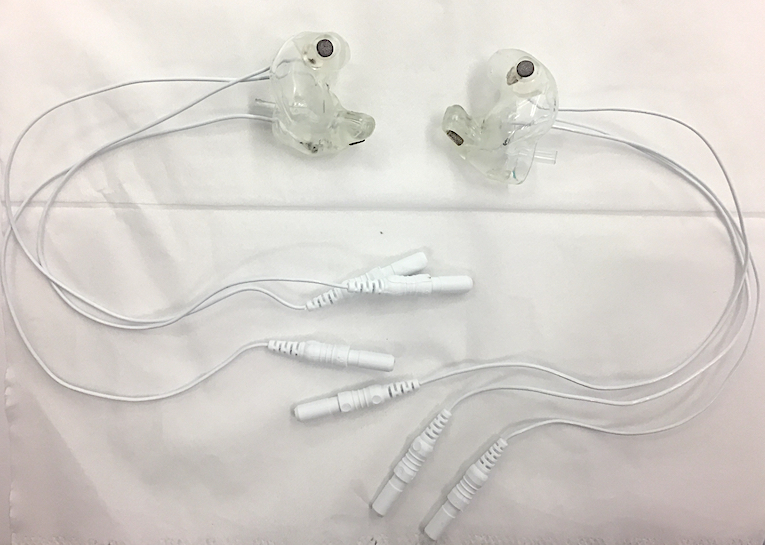
\includegraphics[width=0.5\textwidth]{2EEEG.jpg}
\caption{Pair of custom-fit earpieces with 3 embedded electrodes each located at the helix and front-facing
and back-facing within the ear canal.}
\end{figure}

Research in in-ear EEG is only several years old. Nonetheless, the concept has
attracted a lot of attention because of the discreetness factor of in-ear EEG over
traditional scalp-based EEG. A research team at the Imperial College London
and Aarhus University published a landmark paper in 2011 that introduced the
concept of in-ear EEG, demonstrating for the first time the feasibility of recording
brainwave signals from within the ear canal [11]. Follow-up work from the same
group demonstrated its ability to produce signal-to-noise ratios comparable to
those from conventional EEG electrode placements, robustness to common
sources of artifacts, and use in a brain-computer interface (BCI) system based on
auditory evoked potentials and visual evoked potentials [12-14]. Our own 2016 study
[4] was the first to merge these two streams of work, using in-ear EEG signals for
user authentication with a consumer-grade device. United Sciences is currently
developing a consumer hearable called The Aware that will measure EEG from the ear [15].
Behavioral authentication methods such as keystroke dynamics [16] and speaker
authentication [17] can be categorized as one-step two-factor authentication
schemes. In both cases, the knowledge factor (password or passphrase) and
inherence factor (typing rhythm or speaker’s voice) are employed. In contrast, the
Nymi band [18] supports one-step two-factor authentication via the inherence
factor (cardiac rhythm that is supposed to be unique to each individual) and the
possession factor (the wearing of the band on the wrist). However, as far as we
know, no one has proposed or demonstrated a one-step three-factor
authentication scheme.

\section{Proposed project}
\label{sec:orgb73667f}

We propose the first ever research study on one-step three-factor authentication.
The study will yield a number of novel contributions to the literature. First, we
expect to demonstrate the feasibility of presenting three authenticators in a single
step. Second, we will quantify the performance accuracy of user authentication
using custom-fit in-ear EEG hardware. Third, we can quantify the relative
performance of signals captured from different locations within the ear. Fourth,
we will evaluate the effectiveness of new classes of mental tasks for EEG-based
authentication. Fifth, we will evaluate the usability of custom-fit in-ear EEG
hardware.

\section{Research plan}
\label{sec:orga31e397}

There will be four key components and major research tasks to this proposed
study: (i) design and build custom-fit hardware, (ii) design and implement
authentication tasks, (iii) experimental platform and protocol for data collection,
and (iv) analysis of authentication performance.

In a 2013 passthoughts study [2], unmodified commercial off-
the-shelf EEG sensing hardware was used. In our 2016 Ear-EEG passthoughts study [4],
we modified the off-the-shelf hardware in order to support data collection from
within the ear canal. Once modified, the same device could be used for all
participants. In the current study, we propose to build in-ear EEG sensors that
are custom-fit to the contours of the ears and ear canals of each individual
participant. Therefore, it is necessary for us to build a separate pair of devices for
each participant. In partnership with our research collaborators at Starkey
Hearing Science, who specialize in hearing-aid technologies, we will acquire
moldings of participants’ ears, and use the molds to build custom-fit acrylic
earpieces with embedded EEG electrodes.

A key research challenge is to design and build the electrodes to produce signals
of robust quality, given the small volume of the ear cavity, the small surface
areas of the electrodes, and the limited distances between the electrodes within
the ear. We will need to experiment with the locations of the electrodes, including
the reference and ground electrodes, which may be placed on the ear lobes or
behind the ears on the left and right mastoids.

We propose an update and expansion of the authentication tasks, to take
advantage of our lessons learned from previous studies on the relative strengths
of different mental tasks, with regards to authentication accuracy and usability as
reported by participants. Furthermore, given the in-ear placement of the
electrodes, and hence spatial proximity to the temporal lobes, we see a unique
opportunity to design and test novel authentication tasks based on either auditory
imagery or auditory steady-state response (ASSR). The ten authentication tasks and their
attributes are listed in tables 1 and 2 below.

\begin{table}[h]
\centering
\begin{tabular}{ll}
\textbf{\textbf{Task}} & \textbf{\textbf{Description}}\\
\hline
Breathe & Relaxed breathing with eyes closed.\\
Breathe - Open & Relaxed breathing with eyes open.\\
Sport & Sport-related motor imagery of participant's choice.\\
Song & Imagining a song of participant's choice playing.\\
Song - Open & Imagining a song with eyes open.\\
Speech & Imagining a phrase of participant's choice being spoken.\\
Listen & Tone \& Listening to a continuous tone.\\
Listen - ASSR & Listening to noise modulated at 40 Hz.\\
Face & Imagining a person's face of participant's choice.\\
Sequence & On timed cues, imagine a face, a number, and a word.\\
\hline
\end{tabular}
\caption{Set of tasks proposed for authentication with descriptions.}
\end{table}

\begin{table}[h]
\centering
\begin{tabular}{lllll}
Task & External stimuli? & Personal secret? & Eyes? & Imagery?\\
\hline
Breathe & No & No & Closed & None\\
Breathe - open & No & No & Open & None\\
Sport & No & Yes & Closed & Motor\\
Song & No & Yes & Closed & Aural\\
Song - open & No & Yes & Open & Aural\\
Speech & No & Yes & Closed & Aural\\
Listen - Tone & Yes & No & Closed & None\\
Listen - ASSR & Yes & No & Closed & None\\
Face & No & Yes & Closed & Visual\\
Sequence & Yes & Yes & Open & Visual\\
\hline
\end{tabular}
\caption{Properties of authentication tasks. We selected tasks with a variety of different properteries, but preferred tasks that did not require external stimuli, as the need to present such stimuli at authentication time could present challenges for usability, and user security.}
\end{table}

We will quantify the security and usability performances of these
tasks, both collectively as they contribute to overall authentication accuracy, as
well as comparatively against one another.
We will use OpenBCI, a open-source EEG biosensing system as our data
collection platform. OpenBCI, with a price tag of about \$600,
is an affordable alternative to medical-grade EEG systems that can
cost tens of thousands of dollars. Recent work has demonstrated the robustness 
of OpenBCI compared to an industry standard medical-grade EEG system, 
particularly for non-medical use cases such as the one we propose [26].
Using OpenBCI requires integrating the custom-fit Ear EEG devices with
the OpenBCI board. We will also need to extend our own data collector
software, to support the recording of OpenBCI data that is synchronized with
PsychoPy, which we use for stimuli presentation. We will recruit on the order of
20-30 participants who are willing to commit to multiple session visits, first for ear
molding, then for device impedance testing, and then for one or more data
collection sessions.

For authentication analysis, we will build upon the analysis methodology and
tools from our previous studies. We will apply the logarithmic binning technique
that we have developed in [5] to the EEG power spectrum data during the signal
pre-processing step. We will then apply machine learning to train and test a
support vector classifier as in [4]. We will compare the results against the
threshold-based authentication protocol based on cosine similarity as in [2,3].
A key change for this study is that we will be able to collect up to 8 separate
channels of EEG data, including multiple channels from each ear. This is in
contrast to our previous studies, where we collected only a single channel of
EEG, either on the prefrontal cortex (FP1) location or in the ear canal. Therefore,
we will need to develop new analytic techniques to both (i) assess improvements
in authentication accuracy due to the increased channels of data, and (ii) assess
relative contributions of individual electrode locations to authentication accuracy.
Finally, we will evaluate the usability of custom-fit Ear EEG authentication along
several dimensions. They include the comfort and fit of the earpieces, the
preparatory steps of using the devices, the ease and repeatability of the
authentication tasks, and the recall rates of the personal secrets.
\section{Preliminary results}
\label{sec:org914f392}

We performed a very small pilot study (n=2) to better assess our projects' feasibility,
in particular the new custom-fit ear piece hardware.
Our cursory analysis indicates that we can successfully
detect EEG signals from the ear (Section 5.1), that these signals can be used
for reliable authentication among two people (Section 5.2), and that the success
of the authenticator relies on the user's chosen secret, and not just the inherence
factor of the user's unique signal (Section 5.3).

\subsection{Data collection}
\label{sec:org20a2071}

Our initial participants were recruited from a nearby university and scheduled for ear molding
and impedance checking sessions. Finally, the data collection visit was scheduled and took
approximately 90 minutes for set up and experiment execution. The OpenBCI system we used
allows for 8 channels of simultaneous recording, along with separate ground and reference channels.
Data was initially collected with the ground placed at the center of the forehead, and using the left
mastoid as reference, though we can easily re-reference to another channel by subtracting a desired
channel (such as right mastoid). Each earpiece (shown in the image below) contain three channels: 
one placed on the helix, and two inside the canal - one front-facing and the other back-facing. The remaining
two channels were placed on the right mastoid for later re-referencing, and at approximately Fp1 (on the 
forehead above the left eye) for validating the data collected in the ears against a scalp-based measure. 
Before beginning the experiment, the data from all channels was visualized and participants were asked to
blink and clench their jaws to confirm visibly that all channels were active and properly connected.

During the experiment, participants were seated in a comfortable position in a quiet room facing a laptop screen on which the
instructions and stimuli were presented using PsychoPy. Each task was completed once in sets five trials each, and then
each was completed again for another five trials. Each trial was 10 seconds in length, for a total of 10 trials and 
100 seconds of data collected per task. The instructions were read aloud to the participant by the experimenter, and
the experiment was advanced using a pointer held in the participant's lap to minimize motion artifacts in the data.  
The experimenter also recorded the participant's chosen secrets for the sport, song, face, speech, and sequence
 tasks and reminded the participant of these for the second set of trials.

\subsection{Pilot Data Validation}
\label{sec:org28f05cd}

Using the pilot data from two participants, we were able to confirm the custom-fit earpieces are able to collect EEG
data using three tests: good impedances measured for the ear electrodes, alpha-band activity attenuation when a
participant's eyes were open versus closed, and the presence of a significant ASSR signal.

The recorded impedances of the earpiece electrodes were less than 5 kOhms except one, a benchmark used widely in previous
ear EEG work. The left helix electrode of one participant was measured at 9 kOhms, and generally the 
helix impedances for both participants were higher than their ear canal counterparts. We expected this result, given that the
helix electrode relies on quality of the earpiece's fit outside the ear for good contact, and is not as securely and tightly placed as the
electrodes within the ear canal. Nonetheless, the data from all electrodes were tested in the remaining two data quality tests.

For the alpha-attenuation test, data from the "Breathe" task was compared with that of the "Breathe - Open" task. It is a well-
known feature of EEG data that activity in the alpha-band (approximately 8-12 Hz range) increases when the eyes are closed
compared with a similar state with eyes open. For both of our pilot participants this attenuation is clearly visible even in just
a single trial's data. To further validate, we also performed this calculation on the data collected from the Fp1 electrode and see
the effect clearly here as well. It is important to note that the left ear results are reported using the right mastoid as reference, and
the right ear results in turn using the left mastoid as reference. When using the same side mastoid for reference the effect is not 
visible, though it may be if we average across many trials. This is not surprising, as the further a reference electrode is from the active
channel the less "real" signal is being subtracted from the active channel. This has important design implications for eventual 
real-world deployment of this authentication method however, as it will likely require pieces worn on or around both ears to properly 
function, and not just one. The figures below show the alpha attenuation in the left and right ear channels, as well as Fp1.

\begin{figure}[h]
\centering
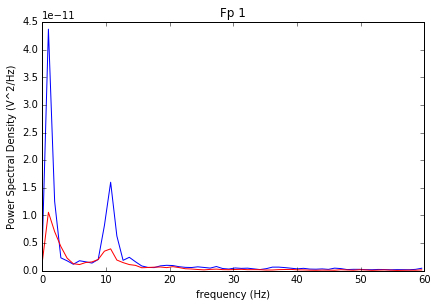
\includegraphics[width=0.5\textwidth]{001_AlphaAtt_Fp1.jpg}
\caption{Alpha-attenuation (8-12 Hz range) in Fp1 channel, referenced at left mastoid, for comparison to ear channels. Red indicates breathing data with
eyes open, blue indicates the same task with eyes closed.}
\end{figure}

\begin{figure}[h]
  \centering
  \begin{minipage}[b]{0.45\textwidth}
    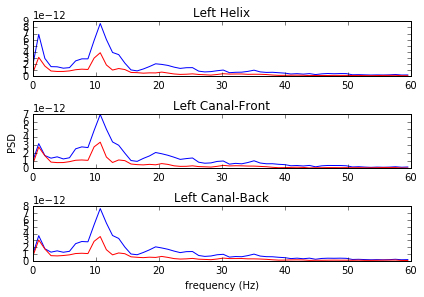
\includegraphics[width=\textwidth]{001_AlphaAtt_Left.jpg}
  \end{minipage}
  \hfill
  \begin{minipage}[b]{0.45\textwidth}
    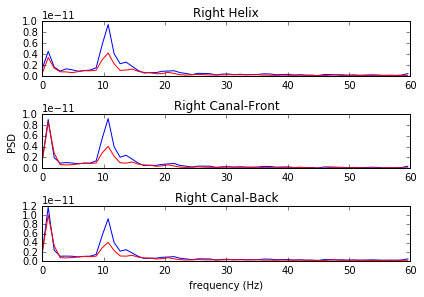
\includegraphics[width=\textwidth]{001_AlphaAtt_Right.jpg}
  \end{minipage}
\caption{Alpha-attenuation (8-12 Hz range) in left and right ear canal channels, referenced at opposite mastoids respectfully. Red indicates breathing data with
eyes open, blue indicates the same task with eyes closed.}
\end{figure}

Finally, for the ASSR test we calculated power spectra for data from the "Listen - ASSR" task. The audio stimulus used for this task is modulated 
at 40 Hz, which should, in turn, produce an EEG response visible in the data at 40 Hz. Strangely, in our tests we do see an ASSR spike but it is located 
around 74 Hz instead. While this has us somewhat perplexed about our stimulus, the purpose of this test was to ensure that the response seen in the ear channels 
matched the response seen from the Fp1 recordings, which is evident comparing the figures below.

\begin{figure}[h]
\centering
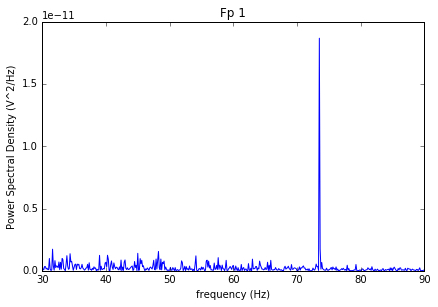
\includegraphics[width=0.5\textwidth]{001_ASSR_Fp1.jpg}
\caption{Power spectrum for data collected from the Fp1 channel during 40 Hz ASSR stimulus. An ASSR spike is clearly visible, though not at 40 Hz where it was expected.}
\end{figure}

\begin{figure}[h]
  \centering
  \begin{minipage}[b]{0.45\textwidth}
    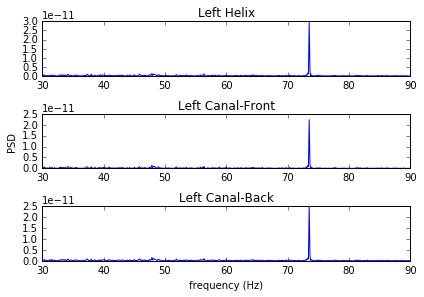
\includegraphics[width=\textwidth]{001_ASSR_Left.jpg}
  \end{minipage}
  \hfill
  \begin{minipage}[b]{0.45\textwidth}
    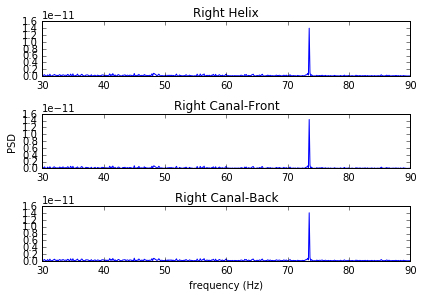
\includegraphics[width=\textwidth]{001_ASSR_Right.jpg}
  \end{minipage}
\caption{Power spectra for data collected from the earpiece channels during 40 Hz ASSR stimulus. Again, the spike is clearly visible though not at 40 Hz, however it 
does match the activity measured at Fp1.}
\end{figure}

\subsection{Authentication performance}
\label{sec:orgfc9b24a}

Following [5], we use logarithmic binning to produce
compressed feature vectors of a variable size. This technique
has been show to offer robust, linear classifiability in healthy
subjects. It is unique in its use of the entire frequency
spectrum. Since EEG activity is primarily associated with frequencies
from 1-40Hz, we presume this range contains the majority of
relevant signal. However, we do not rule out the possibility
that useful signal exists in other frequency ranges. Slight muscular
activity, for example, might be correlated with mental gestures
in some cases. Logarithmic binning produces feature vectors
biased toward known sources of signal, while still including
data points from outside this frequency range that may be
informative.

We analyzed the EEG signals collected during the tasks
using a support vector classifier (SVC). Since past work has
shown that classification tasks in EEG-based BCI are linear
[25], we used XGBoost, a popular tool for generating
ensemble linear classifiers. For each task, for each participant, 
100 seconds of data were
collected in total across 10 trials of 10 seconds each, 
resulting in 30 samples per participant, per task,
following preprocessing.


\begin{table}[h]
\centering
\begin{tabular}{l|rr|rr|rr}
\textbf{Task} & \textbf{Left Ear} &  & \textbf{Right Ear} &  & \textbf{Fp1} & \\
\hline
 & \textbf{FAR} & \textbf{FRR} & \textbf{FAR} & \textbf{FRR} & \textbf{FAR} & \textbf{FRR}\\
\hline
Breathe & 0 & 0 & 0 & 0 & 0 & 0\\
Breathe - Open & 0.039 & 0 & 0 & 0 & 0 & 0\\
Sport & 0.039 & 0.036 & 0 & 0 & 0 & 0\\
Song & 0 & 0 & 0 & 0 & 0 & 0\\
Song - Open & 0 & 0 & 0 & 0 & 0 & 0\\
Speech & 0 & 0 & 0 & 0 & 0 & 0\\
Listen - Tone & 0 & 0 & 0 & 0.009 & 0 & 0\\
Listen - ASSR & 0 & 0 & 0 & 0 & 0 & 0\\
Face & 0 & 0 & 0 & 0.002 & 0 & 0\\
Sequence & 0 & 0 & 0 & 0 & 0 & 0\\
\end{tabular}
\caption{Authentication accuracy for each sensor position. Left and right ears were a composite of three electrode positions along the helix, front of the ear canal, and back of the ear canal.}
\end{table}

Finally, for each subject, for each task, we trained a binary classifier 
in the following manner: the right subject, performing the right task, were taken
as positive examples. The wrong person, performing any task, were taken as negative
examples. For a random, balanced subsample of those groups, we trained an ensemble
binary classifier with XGboost. For the remainder of the data, we tested the 
classifier's accuracy, measuring the false acceptance rate (FAR) and the false
rejection rate (FRR) (Table 3).

Overall, FAR and FRR were extremely low across the board. The right ear 
performed better than the left ear (possibly because the reference was on
the left ear, thus furthest from the right ear). In line with the 
results of prior work, Fp1 performed better than either the left or the right ear,
achieving perfect FAR and FRR scores on all tasks.

\subsection{Disentangling inherence and knowledge}
\label{sec:orga057897}

Though our classifier's accuracy is strong, we still cannot say that it relies 
on both knowledge and inherence to authenticate the subject. Is it the passthought
that the classifier is authenticating, or do users (or earpieces) simply have characteristic
EEG readings? 

If our classifier \emph{only} relied on inherence, we would expect the right person performing
the wrong task to reliably authenticate with the classifier described in Section 5.2.
In other words, we would expect the FAR for right-person-wrong-task to be the same 
as the FAR for right-person, right-task. We calculated the FAR for each task, and performed
a two-tailed t-test to determine our confidence that this set of FARs was drawn from
from a different distribution from those generated during the right-person, right-task trials.

\begin{table}[h]
\centering
\begin{tabular}{lrrr}
\textbf{Task} & \textbf{Right Ear} & \textbf{Left Ear} & \textbf{Fp1}\\
\hline
Breathe & 0 & 0.240 & 0\\
Breathe - Open & 0.254 & 0.129 & 0\\
Sport & 0.222 & 0.135 & 0\\
Song & 0 & 0.211 & 0\\
Song - Open & 0 & 0.166 & 0\\
Speech & 0.311 & 0.116 & 0\\
Listen - Tone & 0 & 0.333 & 0\\
Listen - ASSR & 0.322 & 0.078 & 0\\
Face & 0.355 & 0.055 & 0\\
Sequence & 0.433 & 0 & 0\\
\hline
\textbf{p-value} & \textbf{*0.0076} & \textbf{*0.009} & N/A\\
\end{tabular}
\caption{FARs for right-person, wrong-task, and p-values corresponding to confidence that these FARs were drawn from the same distribution as from the right-person-right-task trials.}
\end{table}

Our low p-values (Table 4) indicate that the passthought, as well as the inherence
factor associated with the custom-fit EEG earbud, both contribute to the classifier
performance discussed in Section 5.2. We are confident, then, in our claim that this work
could potentially yield multiple-factor authentication in a single step. However, we
will need to collect a great deal more data to substantiate this claim rigorously.

\section{Proposed Future Work}

In expanding on the feasibility study we describe above, 
our first task comprises of collecting data from more subjects,
ideally for a subject population of 30.
In addition, we hope to collect more diverse data,
by taking regular samples over a period of a few weeks,
and in a variety of circumstances. Our goal here is to gauge the stability
of EEG readings over time, and outside of lab environments.
If the system will need to be calibrated occasionally, these readings
could help us understand how frequently such calibration sessions
might need to take place.

\subsection{Evaluating a Closed-loop Passthought Authenticator}
Toward this end, propose to build a working, real-time passthought authenticator.
After performing an initial calibration setup, similar to our pilot study's protocol, above,
we will send subjects home with their custom-fit ear EEG, and ask them to use the device to authenticate
two to three times a day for a week.
(We may ask subjects to set a recurring event on their calendar to remind them, 
or pay subjects in accordance with how frequently they authenticated, up to some reasonable maximum).

After a week, subjects will return to the lab to return their equipment, debrief about their experience, and receive payment. We will use this opportunity to walk subjects through a relatively detailed post-interview,
during which we will focus on their experiences with the device. 
The goal of this work is to understand both the technical issues facing ear-EEG authentication
(Does the system work reliably? When and why does it fail?), and the usability issues
(How do subjects feel about having an EEG device in their ear throughout the day?).
Finally, this closed-loop BCI system could help us understand how learning effects
on the human side might impact authentication performance, as the human and machine
co-adapt during multiple authentication attempts.

\subsection{Adding a Third Factor of Authentication}
After testing that our system can reliably provide authentication with a 
a secret passthought (knowledge) and unique EEG signal (inherence),
we will turn our attention to the final, third factor: possession
(of the unique, custom-fit ear EEG device).
We propose to cryptographically assure device possession
by assigning each custom-fit electrode a unique public/private keypair. 
User accounts could be associated with an earpiece's public key,
and authentication attempts from the earpiece could be signed its
its private key, producing authentication attempts that are not
forgeable by other custom-fit earpieces. 

\section{Conclusion}
At the end of the proposed project,
we will have developed an authentication attempt that provides three factors
(knowledge, inherence and possession) in a single authentication attempt.
This work could lead to authentication strategies that are both more secure
and more useable than traditional, password-based authentication.

\section{Proposed Budget}
\label{sec:org7b5c0f3}
With two graduate students working on the project and a target sample size of 30 participants
we propose the following budget:

\begin{itemize}
\item 2x 8-Channel OpenBCI Systems: \$1,200.00 (\$600.00 each)
\item 30x Pairs of custom-fit earpieces with 3 embedded electrodes including labor cost: \$5,100.00 (\$170.00 per pair)
\item 30x Compensation for two visits per participant: \$2,400.00 (\$80.00 each)
\item 2x Graduate student support for two years: \$144,000.00 (\$72,000.00 each)
\item Travel and registration costs for conferences: \$6,000
\item \textbf{Total: \$158,700.00}
\end{itemize}

\section{Group Member Contributions}
Work for this project was approximately split evenly between the two group members. Both group members were involved in the project
ideation and literature review, preparation of initial and final presentations, and preparation of this final proposal. Individually, Max created
the experimental stimulus in PsychoPy and carried out the initial data collection of the pilot participants with some support from Nick. Max 
also ran the alpha-attenuation and ASSR data validation analyses. Along with assisting in data collection, Nick developed and ran the machine
 learning authentication analyses on our pilot data.

\section{References}
\label{sec:org0b0b225}
\setlength\parindent{0pt}

[1]
J. Chuang, One-Step Two-Factor Authentication with Wearable Bio-Sensors, Workshop on
"Who are you?! Adventures in Authentication" (WAY'14), 10th USENIX Symposium on
Usable Privacy and Security (SOUPS'14), 2014.
\hspace{0pt} \\

[2]
J. Chuang, H. Nguyen, C. Wang, B. Johnson, I Think, Therefore I Am: Usability and
Security of Authentication Using Brainwaves, Workshop on Usable Security (USEC'13),
17th Int. Conference on Financial Cryptography and Data Security (FC’13), 2013.
\hspace{0pt} \\

[3]
B. Johnson, T. Maillart, J. Chuang, My Thoughts are Not Your Thoughts: Robustness of
Brainwave Signal Authentication Against Impersonation Attacks, Workshop on Usable
Privacy \& Security for wearable and domestic Ubiquitous Devices, ACM UbiComp, 2014.
\hspace{0pt} \\

[4]
M. Curran, J. Yang, N. Merrill, J. Chuang. Passthoughts Authentication with Low Cost
EarEEG. Proc. 38th Intl. Conf. of IEEE Engineering in Medicine and Biology Society
(EMBC 2016), Aug. 2016.
\hspace{0pt} \\

[5]
N. Merrill, Maillart, Johnson, J. Chuang, Improving Physiological Signal Classification Using
Logarithmic Quantization and a Progressive Calibration Technique, Proc. 2nd Intl. Conf. on
Physiological Computing Systems (PhyCS'15), Feb. 2015.
\hspace{0pt} \\

[6]
J. Thorpe, P. van Oorschot, and A. Somayaji. Pass-thoughts: Authenticating with our
minds. In Proceedings of the New Security Paradigms Workshop (NSPW), 2005.
\hspace{0pt} \\

[7]
M. Poulos, M. Rangoussi, N. Alexandris, and A. Evangelou. Person identification from the
EEG using nonlinear signal classification. Methods of Information in Medicine, 2002.
\hspace{0pt} \\

[8]
S. Marcel and J. del R. Millan. Person authentication using brainwaves (EEG) and
maximum a posteriori model adaptation. IEEE Transactions on Pattern Analysis and
Machine Intelligence, 29(4), April 2007.
\hspace{0pt} \\

[9]
R. Palaniappan. Two-stage biometric authentication method using thought activity brain
waves. International Journal of Neural Systems, 18(1):59–66, 2008.
\hspace{0pt} \\

[10]
C. Ashby, A. Bhatia, F. Tenore, and J. Vogelstein. Low-cost electroencephalogram (EEG)
based authentication. In Proc. of 5th Int. IEEE EMBS Conf. on Neural Engineering, 2011.
\hspace{0pt} \\

[11]
D. Looney, C. Park, P. Kidmose, M. L. Rank, M. Ungstrup, K. Rosenkranz, and D. P.
Mandic, “An in-the-ear platform for recording electroencephalogram,” in Proc. Int. Conf.
IEEE Eng. Med. Biol. Soc., 2011, pp. 6682–6885.
\hspace{0pt} \\

[12]
D. Looney, P. Kidmose, C. Park, M. Ungstrup, M. Rank, K. Rosenkranz, and D. Mandic,
“The in-the-ear recording concept,” IEEE Pulse, vol. 3, no. 6, pp. 32–42, Nov./Dec. 2012.
\hspace{0pt} \\

[13]
P. Kidmose, D. Looney, M. Ungstrup, M.L. Rank, D.P. Mandic, “A study of evoked
potentials from ear-EEG,” IEEE Trans. Biomed. Eng. 60(10), pp. 2824–2830, 2013.
\hspace{0pt} \\

[14]
P. Kidmose, D. Looney, and D. P. Mandic, “Ear-EEG from generic earpieces: a feasibility
study,” in Proc. Int. Conf. IEEE Eng. Med. Biol. Soc., 2013, pp. 543-546.
\hspace{0pt} \\

[15] The Aware. \url{http://efitaware.com} [Online; accessed 22-Oct-2016].
\hspace{0pt} \\

[16] F. Monrose and A. Rubin. Authentication via keystroke dynamics. In Proceedings of the 4th
ACM conference on Computer and communications security, pages 48–56. ACM, 1997.
\hspace{0pt} \\

[17]
K. Stevens et al. Speaker authentication and identification: a comparison of spectrographic
and auditory presentations of speech material. The Journal of the Acoustical Society of
America 44.6 (1968): 1596-1607.
\hspace{0pt} \\

[18] Nymi. \url{https://nymi.com} [Online; accessed 22-Oct-2016].
\hspace{0pt} \\

[19] E. Strickland. In-Ear EEG Makes Unobtrusive Brain-Hacking Gadgets a Real Possibility.
IEEE Spectrum, 7/7/2016.
\hspace{0pt} \\

[20]
N. Merrill, M. Curran, J. Yang, J. Chuang. Classifying Mental Gestures with In-Ear EEG.
Proc. 13th IEEE Intl. Conf. on Wearable and Implantable Body Sensor Networks (BSN
2016), Jun. 2016.
\hspace{0pt} \\

[21]
E. Sedenberg, J. Chuang, D. Mulligan. Designing Commercial Therapeutic Robots for
Privacy Preserving Systems and Ethical Research Practices Within the Home. Intl. J. of
Social Robotics, Aug. 2016.
\hspace{0pt} \\

[22] E. Sedenberg et al. A Window into the Soul: Biosensing in Public. Under review, 2017.
\hspace{0pt} \\

[23] R. Wong et al. “All that happens must be known”: Eliciting Values and Conceptions of
Privacy using Science Fiction. Under review, 2017.
\hspace{0pt} \\

[24]
R. Wong et al. Real-Imaginary Entanglements: Using Science Fiction and Design Fiction to
Explore and Question Sensing and Tracking Technologies. Under review, 2017.
\hspace{0pt} \\

[25] D. Garrett, D. Peterson, C. Anderson, and M. Thaut, “Comparison
of linear, nonlinear, and feature selection methods for eeg
signal classification,” IEEE Transactions on Neural Systems and
Rehabilitation Engineering, vol. 11, no. 2, pp. 141–144, Jun. 2003.
[Online]. Available: \url{http://ieeexplore.ieee.org/lpdocs/epic03/wrapper}.
htm?arnumber=1214704
\hspace{0pt} \\

[26] Frey, Jeremy. "Comparison of an open-hardware electroencephalography amplifier with medical
grade device in brain-computer interface applications." arXiv preprint arXiv:1606.02438 (2016).
\hspace{0pt} \\

\end{document}
